%Descrição do processo de garantia da qualidade do projeto e do produto desenvolvido incluindo:
%   Padrões de referência a serem utilizados/ check lists
%   Processos
%   Auditorias
%   Ações em caso de Não Conformidade
%   Ferramentas da qualidade
%Identificação dos indicadores de qualidade do projeto 
%Descrição do processo de verificação da qualidade do projeto
%   Métodos de verificação
%   Frequência das ações de controle
%   Eventos listados na Matriz de Comunicações
%   Remete ao Controle Integrado de Mudanças em caso de divergência planejado x realizado
%   Plano de ações corretivas e preventivas
%Descrição do processo de verificação da qualidade do produto
%   Métodos de verificação
%   Frequência das ações de controle
%   Eventos listados na Matriz de Comunicações
%   Remete ao Controle Integrado de Mudanças em caso de divergência planejado x realizado 
%   Plano de ações corretivas e preventivas

\chapter{Plano de gerenciamento da qualidade}

\section{Responsabilidades na garantia da qualidade}

%\todo[inline,color=red]{Terminar definição dos responsáveis pela garantia da qualidade.}

\begin{table}[H]
	\begin{tabularx}{\textwidth}{| c | X |}
		\hline
		\textbf{Papel}     & \textbf{Responsabilidade}                            \\
		\hline
		Gerente de projeto & Especificar o cronograma do projeto incluindo testes \\
		\hline
		Desenvolvedores & Desenvolver e realizar testes unitários  \\
		\hline
		Analistas de Testes & Definir os testes necessários e realizar testes de integração \\
		\hline
	\end{tabularx}
	\centering
	\caption{Tabela de responsabilidades na garantia da qualidade.}
\end{table}

\section{Responsabilidades no controle da qualidade}

%\todo[inline,color=red]{Terminar definição dos responsáveis pelo controle da qualidade.}

\begin{table}[H]
	\begin{tabularx}{\textwidth}{| c | X |}
		\hline
		\textbf{Papel}     & \textbf{Responsabilidade}                            \\
		\hline
		Gerente de projeto & Especificar o cronograma do projeto incluindo testes \\
		\hline
		Analista de testes & Coletar e gerenciar os dados resultantes dos testes. \\ %Coletar indicadores de métricas de qualidade. \\
		\hline
		Equipe do Projeto & Realizar reuniões para levantar sugestões de melhoria no processo. \\
		\hline
	\end{tabularx}
	\centering
	\caption{Tabela de responsabilidades no controle da qualidade.}
\end{table}

\section{Processo de gerenciamento da qualidade}

O processo de gerenciamento da qualidade deve seguir o fluxo mostrado na figura \ref{img:quality-management-process}.

\begin{figure}[h]
	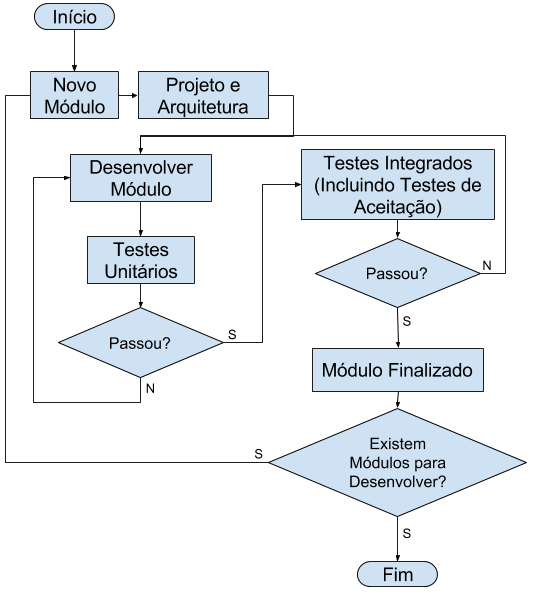
\includegraphics[width=\textwidth]{images/processo-gerenciamento-qualidade}
	\label{img:quality-management-process}
	\caption{Processo de gerenciamento da qualidade.}
\end{figure}

\section{Política de gerenciamento da qualidade}

\begin{itemize}
	\item O sistema de controle de mudanças da qualidade deve ser utilizado para verificar e classificar alterações nos requisitos de qualidade.
	\item Mudanças corretivas que impactem no sucesso do projeto serão incorporadas ao plano.
	\item Todas as solicitações de mudanças devem ser realizadas de acordo com o plano de gerenciamento das mudanças (ver capítulo \ref{ch:change-management-plan}).
\end{itemize}

\section{Planejamento de avaliação de qualidade}

O planejamento de avaliação de qualidade seguirá conforme a tabela \ref{tab:quality-evaluation-plan}.

\begin{table}[h]
	\begin{tabularx}{.9\textwidth}{| c | X | X |}
		\hline
		\textbf{Data} & \textbf{Tipo de Avaliação a ser Realizada} & \textbf{Atividades ou Artefatos a serem Revisados} \\
		\hline
		01/08/2017    & Teste Unitário                              & Aplicativo do Motorista                            \\
		\hline
		14/08/2017    & Teste Unitário                              & Aplicativo do Estacionamento                       \\
		\hline
		21/08/2017    & Teste Unitário                              & Software de Centralização                        \\
		\hline
		01/09/2017    & Teste de Integração                        & Aplicativo do Motorista                            \\
		\hline
		30/08/2017    & Teste de Integração                        & Aplicativo do Estacionamento                       \\
		\hline
		03/10/2017    & Teste de Integração                        & Software de Centralização                        \\
		\hline
	\end{tabularx}
	\centering
	\caption{Planejamento de avaliação de qualidade.}
	\label{tab:quality-evaluation-plan}
\end{table}

\section{Planejamento de testes/inspeções}

\subsection{Configuração do ambiente de teste}

\begin{description}
	\item[Plataforma em Nuvem] \hfill
	\begin{itemize}
		\item Plataforma em nuvem com suporte ao SGBD MySQL.
		\item Plataforma em nuvem para disponibilizar aplicativos web.
	\end{itemize}
\end{description}

\begin{description}
	\item[Dispositivo Móvel] \hfill
	\begin{itemize}
		\item Android v4.0 ou superior.
	\end{itemize}
\end{description}

\subsection{Pré-requisitos}

\begin{itemize}
	\item Conhecimento de abordagens e técnicas de teste.
	\item Conhecimento da aplicação e de seu estado.
	\item Conhecimento de negócio e método de utilização do sistema.
	\item Capacidade de resolução de problemas.
\end{itemize}

\section{Frequência de atualização do plano de gerenciamento da qualidade}

Os requisitos de qualidade do projeto devem ser avaliados semanalmente durante a reunião do CCM, prevista no plano de gerenciamento das comunicações.

\section{Alocação financeira das mudanças nos requisitos de qualidade}

As mudanças nos requisitos de qualidade podem ser alocadas dentro das reservas gerenciais do projeto.

Em caso de mudanças prioritárias nos requisitos de qualidade do projeto, quando não existem reservas gerenciais disponíveis, deverá ser acionado o patrocinador.

\section{Priorização das mudanças nos requisitos de qualidade e respostas}

As mudanças nos requisitos de qualidade deverão ser classificadas de acordo com o modelo de priorização integrada de mudanças (ver seção \ref{sec:integrated-change-priorization}).

\section{Sistema de controle de mudanças da qualidade}

Todas as mudanças nos requisitos de qualidade do projeto devem ser tratados segundo o fluxo apresentado pelo sistema de controle integrado das mudanças (ver seção \ref{sec:change-control-system}).

%\section{Métricas de qualidade}

%As métricas de qualidade encontram-se no apêndice \ref{quality-metrics}.

\section{Administração do plano de gerenciamento da qualidade}

\subsection{Responsável}

\begin{itemize}
	\item \projectManagerName, gerente de projeto, será o responsável direto pelo plano de gerenciamento da qualidade.
\end{itemize}

\section{Outros assuntos relacionados ao gerenciamento da qualidade do projeto não previstos neste plano}

Solicitações não previstas neste plano deverão passar pela aprovação do CCM. Após aprovada o plano deve ser atualizado pelo gerente do projeto.

\section{Controle de Versão}

\begin{table}[H]
	\begin{tabularx}{\textwidth}{| c | c | X | X |}
		\hline
		\textbf{Versão} & \textbf{Data} & \textbf{Autor}      & \textbf{Notas de Revisão} \\
		\hline
		1                &               & \projectManagerName & Criação do documento     \\
		\hline
	\end{tabularx}
	\centering
\end{table}

\section{Aprovações}

\begin{table}[H]
	\begin{tabularx}{\textwidth}{| c | c | X | c |}
		\hline
		\textbf{Função}  & \textbf{Nome}       & \textbf{Assinatura}      & \textbf{Data} \\
		\hline
		Patrocinador       & \projectSponsorName & \projectSponsorSignature &               \\
		\hline
		Gerente de projeto & \projectManagerName & \projectManagerSignature &               \\
		\hline
	\end{tabularx}
	\centering
\end{table}